% !TeX root = ../main.tex

\chapter{A Two-Stage Agentic IP-Reuse Pipeline with Cascade Routing}
\label{ch:03}

This chapter presents the generation methodology of the thesis. Its
core is a two-stage agentic pipeline that generates RTL by first
\emph{planning} which existing IP blocks to reuse and how to integrate
them, and only then generating Verilog under a verify-and-repair loop.
A per-task cascade router completes the methodology by deciding,
before the expensive planning machinery runs, whether a task needs it
at all.

The motivation for the two-stage split is the way large language models
are usually used, and the way that habit fails on tasks of this
scale. The common practice is to hand the model everything at once: the
full specification, every dependency source, and the request for final
code in a single giant prompt. On a RealBench task that one-shot prompt
mixes hundreds of pages of behavioral description with thousands of
lines of provided RTL, and the model must simultaneously decide
\emph{what} to build, \emph{what already exists}, and \emph{how to write
it}. These competing objectives confuse one another and strain the
context window, and the interface details that matter most end up
buried in the middle of it. Separating the work into a planning stage (decide the
reuse and integration structure over a compact, interface-centric view)
and a generation stage (write one module against an already-resolved
plan) gives each LLM call a single objective and a prompt shaped for
exactly that objective. The separation is better on both axes we care
about. It improves accuracy, because each stage sees the right information at the
right altitude, and efficiency, because the expensive full-context
reasoning happens once in the plan rather than being re-derived in
every sample and repair turn.

Section~\ref{sec:pipeline-overview}
gives the dataflow and the environmental contracts the pipeline must honor.
Sections~\ref{sec:pipeline-planner} and~\ref{sec:pipeline-generator} describe
the two stages. Section~\ref{sec:pipeline-repair} describes the three repair
mechanisms layered on the generator --- the syntax repair loop with a
semantic repair cache, the functional repair loop, and diagnostic-driven
specification slicing. Section~\ref{sec:pipeline-routing} presents the
cascade router that chooses per task between this planning flow and a cheap
direct flow. Design decisions are motivated here; their empirical
evaluation is deferred entirely to Chapter~\ref{ch:05}.

\section{Overview and Environmental Contracts}
\label{sec:pipeline-overview}

The pipeline processes one benchmark task end-to-end as follows
(Figure~\ref{fig:intro-overview}):

\begin{enumerate}
  \item \textbf{Catalog construction.} The dependency sources that the
    evaluation environment provides for the task are indexed into a
    per-task \emph{reusable-IP catalog}, with one entry per provided module
    carrying its name, port list, and source. The catalog is the
    pipeline's model of what the test environment supplies, and every
    downstream reuse decision is expressed in its vocabulary.
  \item \textbf{Routing.} The cascade router
    (Section~\ref{sec:pipeline-routing}) reads the specification and
    decides which flow the task takes. Integration-shaped tasks run
    the planning flow of steps 3--5; narrow self-contained tasks skip
    straight to step~5 and generate from the specification alone.
  \item \textbf{Planning.} The planner (Section~\ref{sec:pipeline-planner})
    reads the specification and the catalog and emits a structured IP-reuse
    plan consisting of requirements, module decomposition, a reuse decision per submodule
    (reuse a catalog entry vs.\ write new RTL), and integration notes.
  \item \textbf{Plan adaptation.} An adapter normalizes the plan, resolves
    each reuse decision to concrete source code, and assembles the
    generation prompt from the original specification, the signatures of reused
    modules, environment notes, and the testbench's DUT instantiation, taken
    verbatim as the binding interface contract.
  \item \textbf{Generation and repair.} The generator
    (Section~\ref{sec:pipeline-generator}) produces the target module and
    iterates under an internal Verilator lint that compiles the generated
    code against the same file set the benchmark will use, feeding
    diagnostics back as repair prompts (Section~\ref{sec:pipeline-repair}).
  \item \textbf{Evaluation.} The final candidate is scored by the untouched
    RealBench Makefile as described in Section~\ref{sec:setup-realbench}.
\end{enumerate}

\paragraph{The two fatal contracts.}
Two properties of the evaluation environment shape nearly every design
decision downstream, and both are fatal when violated. First, the
environment compiles \emph{every} Verilog file in the task directory
together, so any provided dependency module that the generated code
re-declares produces a duplicate-module error (\texttt{MODDUP}). Shipped
dependencies must be \emph{instantiated, never re-implemented}. (The single
family-wide exception, \texttt{e203\_extend\_csr}, is not shipped as a file
and must be inlined --- the kind of irregularity that motivates grounding
plans in the real catalog rather than in the model's memory.) Second, the
testbench instantiates the device under test with an exact port list; a
generated module that misses one port fails with \texttt{PINNOTFOUND}
regardless of how correct its internals are. The pipeline addresses the
first contract by stripping re-declared modules and cataloging what is
provided, and the second by injecting the testbench's DUT instantiation into
every generation and repair prompt as a hard interface contract.

\section{Stage One: The Grounded Planner}
\label{sec:pipeline-planner}

The planner is a tool-calling agent. It plans by interacting with a suite
of IP-reuse tools scoped to the per-task catalog, and returns a structured
JSON plan with a fixed schema --- requirement summary, module
decomposition, per-module reuse decisions (\texttt{selected\_ip} naming a
catalog entry, or \texttt{new\_rtl\_required}), and integration,
verification, and debugging plans. Figure~\ref{fig:planning-flow} shows
the stage's dataflow.

\begin{figure}[htbp]
  \centering
  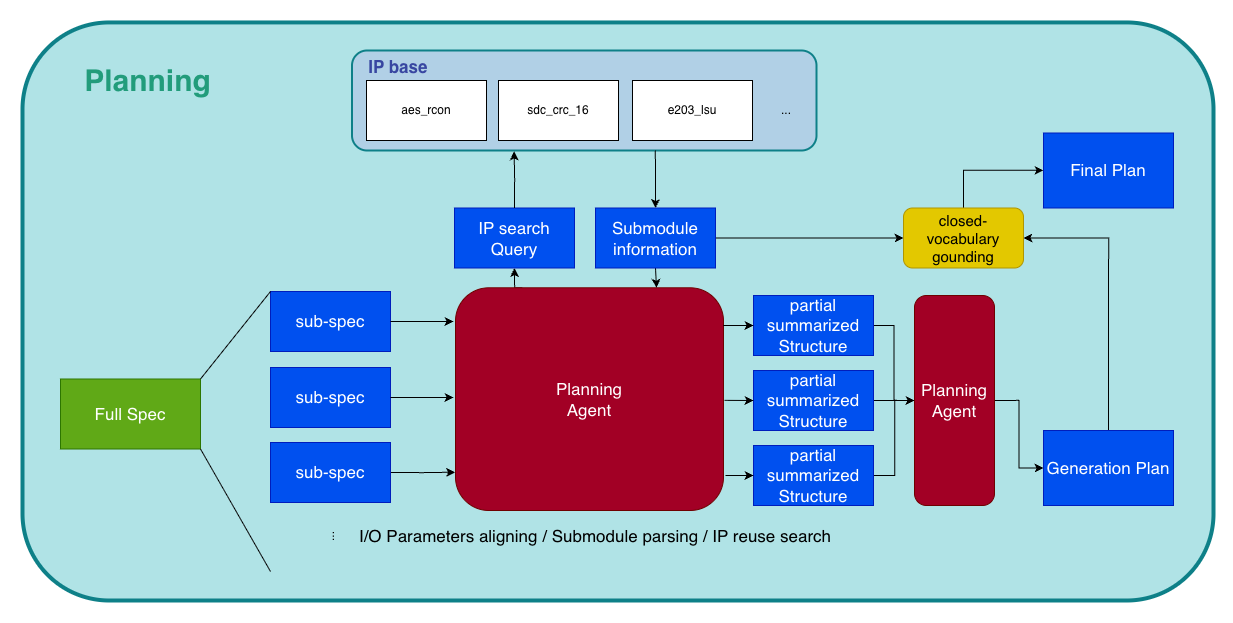
\includegraphics[width=\textwidth]{figures/planning-new.png}
  \caption[Planning stage dataflow]{Dataflow of the planning stage.
    Large specifications are split into sub-specs and summarized
    chunk-by-chunk into partial structured summaries (the condensation
    described later in this section). While planning, the agent
    queries the per-task IP catalog and reads back submodule interface
    information, and a merge pass turns the partial summaries into the
    generation plan. Closed-vocabulary grounding then resolves every
    reuse decision against the catalog and releases the final plan to
    the generator.}
  \label{fig:planning-flow}
\end{figure}

\paragraph{The IP-reuse tool suite.}
Four tools carry the reuse workflow. \texttt{search\_reuse\_ip} queries
the per-task catalog for candidate modules (token-overlap,
semantic-embedding, or hybrid retrieval backends, selected by
\texttt{--planner-search-mode}); \texttt{inspect\_reuse\_ip} returns one
candidate's behavior, interfaces, parameters, limits, and integration
notes; \texttt{evaluate\_ip\_candidate} scores a candidate on function
match, interface compatibility, configurability, and verification
status; and \texttt{check\_port\_compatibility} parses port declarations
and verifies that a proposed instantiation's connections are legal.
Auxiliary tools (\texttt{write\_artifact}, \texttt{generate\_rtl\_module},
\texttt{validate\_verilog}) let the agent persist plan artifacts and
sanity-check RTL sketches. The intended interaction per submodule is
search~$\to$ inspect~$\to$ evaluate~$\to$ decide. The agent searches the
catalog with a behavioral query, inspects the top candidates' interfaces,
scores the fit, and only then commits the submodule to a reuse decision.

\paragraph{Reuse or new RTL.}
The per-module decision between \texttt{selected\_ip} and
\texttt{new\_rtl\_\allowbreak required} is the plan's load-bearing output, and its
two error directions cost very differently. Declaring reuse of a module
that does not fit (or does not exist under that name) is fatal
downstream. The generator either re-implements a shipped dependency
(\texttt{MODDUP}) or instantiates a phantom (\texttt{MISSING-MODULE}),
both of which kill the sample at compile time. Missing a legitimate
reuse is gentler but wasteful. The generator re-derives, from prose,
logic that already exists in verified form --- exactly the work IP reuse
is meant to eliminate --- and every re-derived line is a fresh
opportunity for functional error. The decision rule therefore leans on
evidence. A submodule is marked \texttt{selected\_ip} only when a
catalog entry matches both its function and its interface obligations,
and \texttt{new\_rtl\_required} otherwise. The grounding mechanisms
below guarantee that whichever path produced the name, it resolves to
a real catalog entry. Because the environment ships dependencies as
files, reuse decisions also determine prompt composition. Reused
modules enter the generation prompt as interfaces to instantiate,
and new-RTL modules as behavioral requirements to implement.

Three mechanisms make the plan's grounding independent of any single
step of the agent's trajectory --- whatever mixture of tool evidence and
direct reading produced a decision, the result is checked against the
catalog. Together we call them \emph{grounding-by-construction}:

\begin{enumerate}
  \item \textbf{Catalog injection.} The real catalog vocabulary --- every
    reusable module id with a one-line digest --- is injected directly into
    the planner's prompt, and the system prompt mandates a closed
    vocabulary in which \texttt{selected\_ip} must be one of the listed ids.
  \item \textbf{Closed-vocabulary grounding.} Every \texttt{selected\_ip} in
    the returned plan is post-hoc resolved against the catalog: exact
    matches kept; near misses remapped by prefix/substring matching and then
    fuzzy string similarity (cutoff 0.6); irrecoverable names dropped and
    the submodule marked \texttt{new\_rtl\_required}. The plan also
    records the grounding outcome per decision, making plans auditable.
  \item \textbf{Completeness gate.} A task whose catalog is non-empty but
    whose plan contains no reuse and no integration content is re-prompted
    once, and the more complete of the two attempts is kept.
\end{enumerate}

Chapter~\ref{ch:05} (Section~\ref{sec:results-grounding}) audits the effect.
Grounding eliminates hallucinated names from plans entirely, making every
plan \emph{correct and auditable}, while the end-to-end pass rate stays
essentially level. The generator was already robust to imperfect names
downstream, so the gain lands in plan quality and auditability rather
than in raw yield.

\paragraph{Large specifications.}
Specifications beyond a token threshold (45{,}000 estimated tokens) are
condensed before planning by a chunk-and-merge summarizer that renders two
views from one manifest: a \emph{planner view} (interfaces, reuse queries,
and a brief behavioral digest) and a \emph{generation view} (full
requirements for to-be-generated logic; interface-only for provided IP).
Port tables and module headers are carried \emph{verbatim} from the raw
specification past the LLM summarizer, because interface fidelity is exactly
what the two fatal contracts punish. Condensation compresses the largest
specifications by roughly $5\times$ (e.g., $\sim$720\,k $\to$ $\sim$146\,k
characters) while keeping every shared fact and module interface stated
exactly once.

\section{Stage Two: The Generator}
\label{sec:pipeline-generator}

The generator receives the adapted plan and produces the target module with
a code-focused prompt assembled from the (possibly condensed) specification;
the source and signatures of every reused module; the environment notes
(which modules are provided as files, which macros the environment defines);
and the testbench DUT instantiation as the interface contract. Generated
text is parsed for a Verilog code block; provided dependency modules that
the model re-declared anyway are stripped before verification. The full
prompt template is reproduced in Appendix~\ref{app:prompts}.
Figure~\ref{fig:codegen-flow} shows the stage's dataflow, including the
repair machinery that Section~\ref{sec:pipeline-repair} describes.

\begin{figure}[htbp]
  \centering
  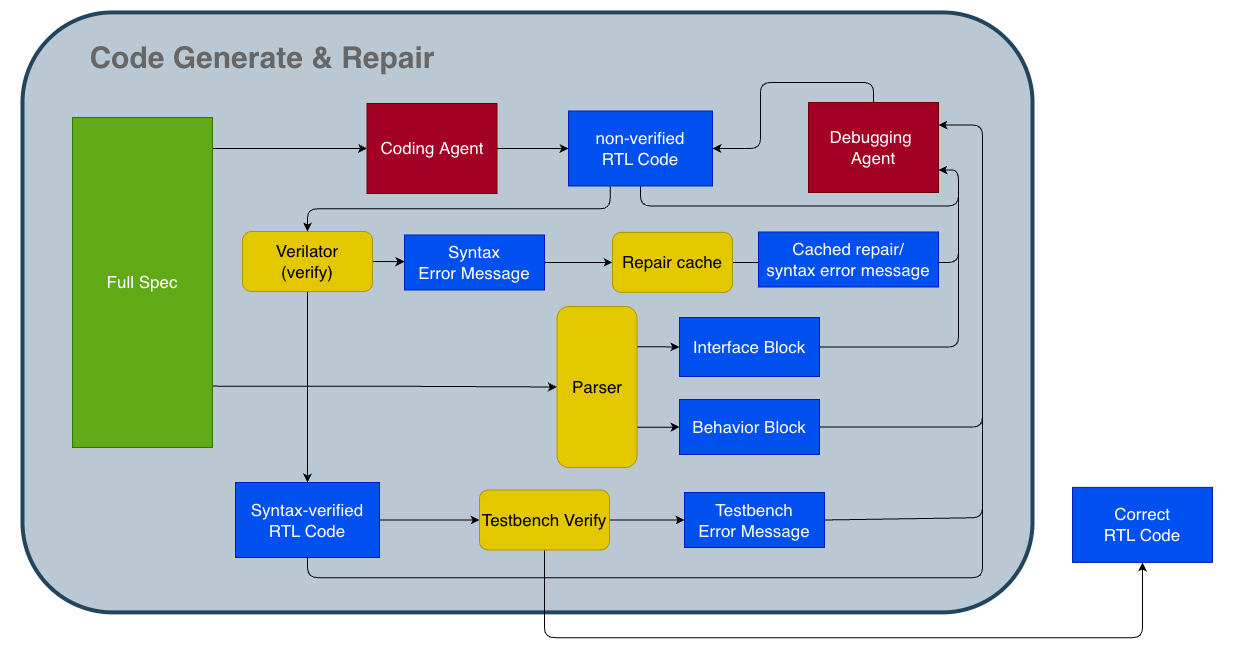
\includegraphics[width=\textwidth]{figures/code-gen-new.png}
  \caption[Generation and repair dataflow]{Dataflow of the generation
    and repair stage. The coding agent produces a candidate module,
    which Verilator lints against the same file set the benchmark
    compiles. Lint diagnostics are matched against the semantic repair
    cache and fed, with any cached fix hints, to the debugging agent
    for syntax repair. A parser splits the specification into
    interface- and behavior-topic slices; the interface slice feeds
    syntax repair and the behavior slice functional repair
    (Section~\ref{sec:pipeline-slicing}). Syntax-verified candidates
    are simulated against the testbench, whose mismatch reports drive
    the functional repair loop (off by default,
    Section~\ref{sec:pipeline-funcrepair}). The surviving candidate
    exits as the final RTL. In the planning flow the coding prompt
    additionally carries the final plan
    (Figure~\ref{fig:intro-overview}).}
  \label{fig:codegen-flow}
\end{figure}

\paragraph{Internal verification mirrors the benchmark.}
The generator's inner loop lints each candidate with Verilator against the
\emph{same} file set the benchmark compiles --- dependencies, reference
model, and testbench, with the task Makefile's warning waivers applied ---
rather than linting the generated file in isolation. This design decision
followed a concrete failure. An earlier isolated lint could not see
testbench-side pin connections, so interface violations
(\texttt{PINNOTFOUND}) sailed through internal checks and died only at
evaluation. Mirroring the benchmark's compile closes that gap; on the runs
where both verdicts exist for identical code, the internal lint agrees with
the benchmark's syntax verdict on 60 of 60 tasks. One divergence survives
in the strict direction, however. The gate treats a few warning classes as
fatal that the scoring build never emits, burning repair budget on code
that is not the problem, an artifact quantified in
Section~\ref{sec:results-artifacts}. The cost of this fidelity
is that Verilator diagnostics can quote testbench or reference lines into
repair prompts; we return to this leak surface in
Section~\ref{sec:threats}.

\paragraph{Syntax first, then function.}
The verification order --- establish syntax correctness, then check
function --- is a deliberately robust flow, and it mirrors how an RTL
engineer works. Code that does not compile cannot be simulated, so
functional evidence only exists for compiling candidates. The ordering
also matches the character of the two feedback signals. Syntax
diagnostics are precise, local, and actionable (a file, a line, an
identifier, an error class), so they are worth iterating on first and
cheaply; functional mismatch reports are coarse and global, so they are
spent only on candidates that have already cleared the structural
contracts. Every repair mechanism in the next section is built around
this two-gate structure. Candidates flow through the syntax gate into
the functional gate, and no repair turn ever advances a candidate that
regresses the earlier gate.

\section{Repair Mechanisms}
\label{sec:pipeline-repair}

Three mechanisms sit on top of the generator's inner loop
(Figure~\ref{fig:repair-loop}). Throughout the
thesis, a repair \emph{budget} ``$s/f$'' means at most $s$ syntax-repair and
$f$ functional-repair attempts per sample. The prompt text of both
repair loops is reproduced in Appendix~\ref{app:prompts}.

\begin{figure}[htbp]
  \centering
  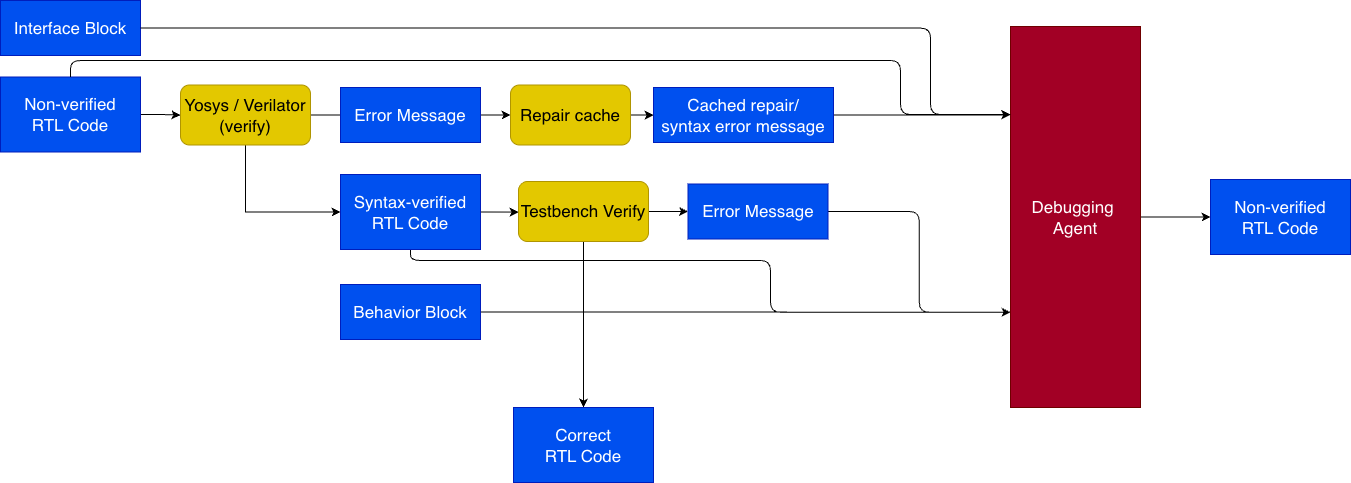
\includegraphics[width=\textwidth]{figures/rep-arch.png}
  \caption[Repair architecture]{The repair architecture. A candidate is
    first verified with Yosys/Verilator; its diagnostics, any similar
    cached repairs (Section~\ref{sec:pipeline-cache}), and the
    specification's interface-topic slice feed the debugging agent. A
    syntax-verified candidate is then simulated against the testbench,
    whose mismatch report and the behavior-topic slice feed the same
    agent (off by default; Section~\ref{sec:pipeline-funcrepair}). The
    agent returns a new candidate that re-enters verification, up to
    the repair budget.}
  \label{fig:repair-loop}
\end{figure}

\subsection{Syntax Repair Loop and the Semantic Repair Cache}
\label{sec:pipeline-cache}

When the internal lint fails, the diagnostics are fed back to the model in a
repair prompt together with the current candidate, and the process repeats
up to the syntax budget. The loop is enhanced by a \emph{semantic repair
cache} that reuses the model's own past
successes. Whenever a repair subsequently \emph{passes} verification, the
pair (diagnostic signature $\to$ unified-diff excerpt of the fix) is stored.
Signatures are Verilator diagnostic lines with file paths and identifiers
stripped, gated by error code, so that structurally identical errors on
different modules collide. On a later failure, sufficiently similar cached
entries are injected into the repair prompt --- \emph{advisory only}, never
auto-applied, and never sourced from benchmark reference code. The cache
has three scopes: \texttt{off}, \texttt{task} (shared only across one
task's samples), and \texttt{run} (shared across the whole run). Run scope
maximizes hint availability; what each scope buys is measured in
Section~\ref{sec:results-cache}.

\subsection{Functional Repair Loop}
\label{sec:pipeline-funcrepair}

The syntax loop is structurally blind to the largest failure class,
candidates that compile but fail the testbench
(Section~\ref{sec:results-failure}). The functional repair loop attacks
this class directly. After a candidate passes syntax, the testbench is run;
on mismatch, the simulator's mismatch report (``Output \texttt{x} has $N$
mismatches, first at time $T$'') is fed back in a prompt that frames the
problem explicitly as \emph{logic} repair --- the interface is correct, do
not change it. The loop keeps the best \emph{compiling} candidate by
lowest mismatch count and never advances to a candidate that regresses
syntax.

One methodological property makes this loop different in kind from syntax
repair, and we flag it prominently. The feedback signal comes from
\emph{the same testbench that scores the benchmark}. A pass obtained
through functional repair therefore means ``specification plus oracle
feedback,'' not ``specification alone.'' For that reason the loop is off
by default and reported as a separate experimental arm
(Section~\ref{sec:results-funcrepair}); headline pipeline-vs-baseline
comparisons never include it.

\subsection{Diagnostic-Driven Specification Slicing}
\label{sec:pipeline-slicing}

Repair prompts initially carried the full specification, which for large
tasks buries the relevant sentence under tens of thousands of irrelevant
tokens. Specification slicing exploits the fact that Verilator diagnostics
and testbench mismatch reports name the offending identifiers exactly. The
slicer extracts those identifiers, then assembles a focused slice. The slice contains the
verbatim interface excerpts (port tables, module headers) plus only the
specification sections that mention an offending identifier, under a
character budget. When a diagnostic names no identifier (e.g., a bare parse
error), the slicer returns nothing and the full specification is kept, so
repair is never starved of context. Interface-topic slices feed the
syntax repair loop, where the errors are overwhelmingly signal-naming and
port-contract issues; behavior-topic slices feed the functional repair
loop, where the model must locate mis-implemented logic.

The compression this buys is large. On the largest specification the
slice is a $\sim$29$\times$ reduction ($\sim$704\,k $\to$ 24\,k
characters). But the reduction rate is only meaningful when read
together with the repair success rate, because a smaller prompt that
dropped the fixing sentence would be a pure regression. The budget calibration of
Section~\ref{sec:results-budget} shows the slice preserves the signal
that matters. With sliced repair prompts, the rescues that occur land
within the first few attempts of both loops, so each rescue is reached
at a fraction of the full-specification token cost per attempt.


\section{Cascade Routing between Direct and Planning Flows}
\label{sec:pipeline-routing}

The planning flow is not the cheapest way to solve every task. Comparing it
task by task with \emph{direct} generation --- a single-shot prompt
with no plan --- shows that the two flows have sharply different
economics. The planning flow's coverage subsumes the direct flow's, but at
an order of magnitude more tokens per sample, and its planning
machinery, decisive on integration problems, is measurably
counterproductive on self-contained algorithm and FSM design, exactly
where the cheap flow matches it. This division matches the purpose of
the thesis. IP-reuse problems mostly need several existing modules
arranged and integrated correctly, which is where the plan pays. The
residual algorithmic tasks are served equally well, and far more
cheaply, by direct generation. The final component of the methodology
is therefore a per-task \emph{cascade router} that predicts, before
planning-scale compute is spent, which of the two flows a task should
take. Section~\ref{sec:router-motivation} establishes why the two
flows are complementary; Section~\ref{sec:router-classes} defines the
task classes and the oracle labels used to evaluate routing; and
Section~\ref{sec:router-design} describes the two-tier cascade and the
metrics it is scored on.

\subsection{Motivation: Two Complementary Flows}
\label{sec:router-motivation}

Running \emph{both} flows on all 60 tasks (the \textsc{Hybrid} arm of
Table~\ref{tab:run-inventory}) motivates routing. With ten samples per
flow, the planning flow solves 20 tasks; the direct flow solves 11 ---
every one of them also solved by the planning flow. Coverage,
then, does not argue for keeping a direct flow at all --- cost does.
Wrapper and integration modules pass only under the planning flow, which
supplies the exact interfaces of the submodules they must instantiate
and wire. Self-contained algorithmic modules pass under direct
generation too, in one coherent piece, at roughly a tenth of a planning-flow
sample's token cost. On exactly those tasks the
planning machinery is measurably counterproductive, as the next
paragraph details. One flow dominates on \emph{ability}; it is far from
dominant on \emph{cost per solved task}.

\paragraph{Why planning is overhead on algorithm/FSM tasks.}
That the planning flow converts poorly on algorithmic and FSM tasks is
measurable in the \textsc{Hybrid} run's own planning flow. On tasks
whose specification centers on a state machine, compiling samples
convert to passes at 16.2\,\%, against 43.1\,\% elsewhere. This is not
an implementation accident; it follows from what planning does. First,
decomposition fragments coherence. A state machine or an arithmetic
datapath is one tightly coupled artifact. A plan that splits it into
submodule pieces forces the generator to implement fragments and glue
where a single \texttt{always}-block idiom --- exactly the pattern the
model knows best from pretraining --- would have expressed the whole
behavior (compiling samples that follow the plan's multi-module
decomposition pass at 12.5\,\%, against 35.3\,\% for single-module
outputs). Second, the plan is a paraphrase. It restates the
specification's behavior in summarized form, and for algorithmic logic
the value lives in exact details (encodings, priorities, edge conditions)
that summarization inevitably coarsens. The generator then optimizes
toward the paraphrase rather than the source. Third, the plan's main
asset --- verbatim submodule interfaces --- is worth little on a task
with nothing to instantiate, so the algorithmic task pays planning's
context and structure overhead without collecting its benefit. Routing
exists to give each task only the machinery it benefits from.

The brute-force deployment --- run both flows on every task --- is the
most expensive one, and it wastes most of its budget. Every direct
sample spent on a wrapper module converts to nothing, and every
planning-flow sample spent on a small self-contained module pays an order of
magnitude more tokens for a task the cheap flow solves equally well. A
router that sends each task to its matching flow can, in principle,
hold the attainable coverage at a fraction of the cost. The routing
problem is to make that prediction \emph{before} the expensive flow has
been paid for.

\subsection{Task Classes and Oracle Labels}
\label{sec:router-classes}

Before formalizing classes, it is worth looking at the two solved sets
concretely rather than only through aggregate rates. In the
\textsc{Hybrid} run, nine tasks pass \emph{only} under the planning flow,
and eleven pass under direct generation as well as under the planning flow
(Table~\ref{tab:flow-sets}). The membership is telling. The
planning-only set is wrappers, memories, and thin glue --- SRAM and
memory wrappers, controller and register-file shims, and the IFU
integrator --- tasks whose difficulty is wiring interfaces the direct
prompt cannot see. The direct-solvable set is small self-contained
modules --- the AES S-boxes and key expansion, the CRC engines, and
clock, CSR, and interrupt utilities --- whose behavior fits in one
coherent piece and offers nothing to reuse.

\begin{table}[htbp]
  \centering
  \caption[Planning-only vs.\ direct-solvable sets]{The planning-only
    and direct-solvable sets of the \textsc{Hybrid} run
    ($60\times(10{+}10)$, ref-hack samples excluded per
    Section~\ref{sec:results-artifacts}), with structural statistics of
    their golden implementations (median / mean / range). ``Own cells''
    = synthesized cells of the module's own logic after subtracting
    submodule instances; regular-array wrappers count as 0, modules
    Yosys cannot elaborate standalone are omitted. Yield counts passing
    samples per solved task in the set's own flow.}
  \label{tab:flow-sets}
  \small
  \setlength{\tabcolsep}{5pt}
  \begin{tabular}{@{}l
      >{\raggedright\arraybackslash}p{0.33\textwidth}
      >{\raggedright\arraybackslash}p{0.38\textwidth}@{}}
    \toprule
     & Planning-only (9 tasks) & Direct-solvable (11 tasks) \\
    \midrule
    Members &
      \texttt{e203\_srams}, \texttt{e203\_itcm\_ram},
      \texttt{e203\_dtcm\_ram}, \texttt{e203\_dtcm\_ctrl},
      \texttt{e203\_exu\_regfile}, \texttt{e203\_exu\_alu\_csrctrl},
      \texttt{e203\_exu\_alu\_rglr}, \texttt{e203\_ifu},
      \texttt{e203\_ifu\_minidec} &
      \texttt{aes\_sbox}, \texttt{aes\_inv\_sbox},
      \texttt{aes\_key\_expand\_128}, \texttt{aes\_rcon},
      \texttt{sd\_crc\_7}, \texttt{sd\_crc\_16},
      \texttt{sd\_fifo\_tx\_filler}, \texttt{e203\_clkgate},
      \texttt{e203\_clk\_ctrl}, \texttt{e203\_extend\_csr},
      \texttt{e203\_irq\_sync} \\
    \midrule
    Code lines        & 114 / 145 / 71--344        & 93 / 121 / 34--323 \\
    Spec size (chars) & 5.4k / 8.9k / 3.6k--26k    & 3.5k / 3.9k / 1.6k--6.8k \\
    Own cells         & 0 / 24 / 0--122            & 20 / 201 / 0--640 \\
    Passing yield     & stable (mean 7.7/10)        & exploratory (mean 4.5/10) \\
    \bottomrule
  \end{tabular}
\end{table}

The structural statistics in Table~\ref{tab:flow-sets} separate the
two sets and make the eventual classifier concrete.
Planning-only modules synthesize to \emph{zero own cells} at the median
--- their logic \emph{is} their submodule wiring --- and carry the
longer, port-table-dominated specifications. Direct-solvable modules
are briefly specified, self-contained, and carry their modest logic
entirely in-house (median 20 own cells, up to 640 for the S-boxes)
with no dominant submodule structure. The two sets also differ in how
they pass. Planning-solved tasks pass stably (7.7 of 10 samples on
average, the interfaces being supplied rather than guessed), while
direct-solved tasks pass by exploring the solution space (4.5 of 10).
These are exactly the observable characteristics --- delegation vs.\
own logic, interface-dominated vs.\ behavior-dominated specification
--- that the router's feature extractor
(Section~\ref{sec:router-design}) is built to read from the
specification alone.

We formalize the division as two task classes:

\begin{description}
  \item[Class A (structural).] Wrapper, integration, and memory-encapsulation
    modules. The module's own logic is thin; its difficulty is wiring
    externally defined submodule interfaces correctly. Class~A tasks want
    the \textbf{planning flow}.
  \item[Class B (algorithmic).] Self-contained datapath or control modules
    --- cipher rounds, CRC, instruction decode, address generation. The
    difficulty is the logic itself, not integration. Class~B tasks are
    the candidates for \textbf{direct} generation --- not because the direct flow solves
    more of them, but because it solves the solvable ones at a tenth of
    the cost while the planning flow's overhead actively hurts.
\end{description}

For evaluation only, each task receives an oracle label computed from its
\emph{golden} implementation. The reference RTL is synthesized with Yosys,
submodule instances are subtracted, and the task is labeled~A if its own
synthesized logic falls below a 250-cell threshold (or it is a recognized
regular-array wrapper), otherwise~B. Oracle labels use golden RTL that
no generation-time component may see; they exist so that routing
decisions can be audited against structure. Class membership alone
does not decide which flow converts a task --- most class-B tasks are
solved by neither flow --- so Section~\ref{sec:results-routing} scores
routing correctness against \emph{empirical flow-solvability}, whether
each task solvable by exactly one flow was routed to that flow.

\subsection{The Two-Tier Cascade}
\label{sec:router-design}

\begin{figure}[htbp]
  \centering
  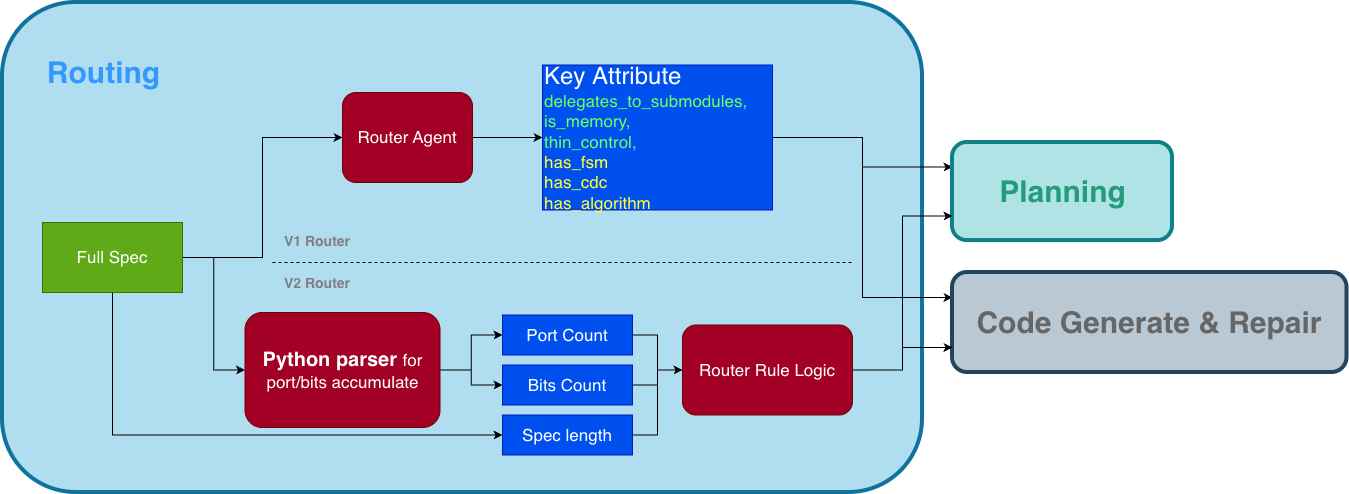
\includegraphics[width=\textwidth]{figures/router-arch.png}
  \caption[Spec pre-route, v1 and v2]{The spec pre-route in its two
    versions. Under the v1 rule the router agent reads the
    specification and emits the key routing attributes ---
    delegation, memory, and thin-control signals for class~A, FSM,
    CDC, and algorithm signals for class~B --- and the decision
    follows from these attributes alone, with an unconfident or
    undecided read falling through to the Tier-1 plan probe. The
    re-derived v2 rule gates deterministically instead. A small
    parser accumulates the port count from the specification's port
    tables and measures the specification length, and the rule logic
    combines these caps with the extractor's delegation judgment and
    own-state-bits estimate. Either way a task exits to the planning
    flow or to direct generation and repair.}
  \label{fig:router-flow}
\end{figure}

The router is a cascade of two increasingly expensive tests; a task
exits at the first tier that is confident.
Figure~\ref{fig:router-flow} shows the first tier in both of its
versions, the v1 read that routes from the extracted key attributes
alone and the re-derived v2 rule that adds deterministic gates parsed
from the specification itself.

\paragraph{Tier-0: spec pre-route.}
A feature extractor reads the specification and emits seven structured
judgments: whether the module delegates to submodules, is a memory
encapsulation, or is thin pass-through control (all class-A signals);
whether it contains a finite-state machine, clock-domain crossing, or a
datapath algorithm (class-B signals); and an estimate of the state bits the
module itself must hold, plus a confidence value. The production extractor
is a small LLM call that returns this JSON verdict (a regex-based keyword
extractor over the same features serves as the ablation baseline ---
Section~\ref{sec:results-routing}). The extractor prompt is reproduced
in Appendix~\ref{app:prompts}. The decision rule is deliberately
transparent and conservative. The planning flow is the default. A task
routes to \emph{direct} only when the extractor reports no submodule
delegation, its substantive logic is a self-contained algorithmic
core, and it passes conservative gates on port count, specification
length, and estimated own-state bits --- the signature of the narrow
computational leaves of Section~\ref{sec:router-classes}. The gates
are deterministic. A small parser counts the specification's
port-table rows and measures its stripped length; only the own-state
estimate comes from the extractor. This gated, planning-default form
is the v2 rule of Figure~\ref{fig:router-flow}. The earlier v1 rule
decided from the extracted attributes alone, releasing any
self-contained-core signal to direct, a polarity
Section~\ref{sec:results-routing} traces to invalidated evidence and
re-derives. When the extractor's confidence is below threshold, or
its attributes leave the class undecided, the task falls through as
\emph{uncertain}.

\paragraph{Why an LLM extractor rather than parsing.}
The features themselves are simple enough that keyword matching looks
tempting, but specification language is \emph{semantically misleading}
at exactly the decision boundary. A module can sound algorithmic while
being structural. \texttt{e203\_ifu\_minidec} is described as
performing ``preliminary decoding,'' yet it is a thin wrapper that
instantiates the real decoder. A keyword extractor reads
``decoding'', sees a self-contained core with no delegation
vocabulary to contradict it, and releases the task to direct
generation, where it has no access to the decoder interface it must
wire. The reverse confusion also occurs.
Specifications for genuinely algorithmic FIFOs and CRC engines spend
most of their text on bus-facing port tables, so surface counting of
interface vocabulary misreads them as structural. Deciding the class
requires reading what the module \emph{does} across the whole document
--- whether the described behavior is delegated or computed --- which is
a semantic judgment, not a lexical one. The whole-spec LLM read resolves
both directions, and the ablation of Section~\ref{sec:results-routing}
quantifies the gap to the keyword baseline.

\paragraph{What the specification cannot decide.}
Not every specification commits its module to either class. Across
the 60 tasks, the extractor returns all-false features at full
confidence for exactly five:
\texttt{sd\_bd} (a buffer-descriptor manager), \texttt{sd\_data\_serial\_host}
(the SD data-line serial engine), \texttt{e203\_biu} (the bus interface
unit), \texttt{e203\_exu\_alu\_lsuagu} (the load/store address-generation
unit sharing the ALU datapath), and \texttt{e203\_exu\_wbck} (the
write-back arbiter). All of them are \emph{interface-arbitration
modules} that sit between protocols. They neither delegate to
submodules (no class-A signal fires) nor implement a nameable algorithm
or FSM (no class-B signal fires), but instead mediate, arbitrate, and
translate between interfaces with modest own state. The specification
genuinely does not commit the module to either class, and only the
plan --- which makes the delegation structure explicit --- can. These
are precisely the tasks the second tier exists for.

\paragraph{Tier-1: plan probe.}
Uncertain tasks run the planner once --- the cheapest informative
component of the planning flow --- and the router probes the resulting structured plan's own
natural-language requirement summary. The plan is a good routing feature
for the same reason the condensation stage renders two views
(Section~\ref{sec:pipeline-planner}). The \emph{planner view} is built
to surface each module's delegation and reuse structure while the
\emph{generation view} carries its full behavioral requirements. By
the time a plan exists, characteristics that were ambiguous in the raw
specification --- does this module instantiate the work or perform it?
--- have been made explicit in the plan's own vocabulary of reuse
decisions and requirement summaries. The probe simply reads that
vocabulary back. Decisive delegation phrasing
(``wraps'', ``encapsulates'', ``reuses existing'', or instantiation language
without any own-implementation verb) keeps the task in the planning flow, plan
in hand; clear self-contained-algorithm phrasing routes it to direct,
\emph{discarding} the plan. The asymmetry of the default is intentional.
The plan is already a sunk cost, so the probe bails to direct only when the
module is clearly self-contained. A plan generated and then discarded is
counted as a \emph{wasted plan} --- the cascade's overhead metric.

\paragraph{The direct flow.}
The direct arm is not a bare completion. It shares the generator's repair
machinery. A directly generated candidate that fails the internal lint
enters the same syntax repair loop, and (in arms where functional repair is
enabled) the same functional repair loop, with the plan-dependent prompt
sections simply absent. This matters for the routing economics. Direct
generation costs roughly 10--12\,k tokens per sample against the planning flow's
90--153\,k, so every correctly-routed class-B task buys nearly an order of
magnitude of compute reduction. Section~\ref{sec:results-routing}
measures the realized economics.

\paragraph{Routing metrics.}
Section~\ref{sec:results-routing} evaluates routing arms on four axes:
\emph{coverage} (solved tasks and pass@k, against the planning flow's
genuine coverage as the attainable ceiling); \emph{routing accuracy}
(against empirical flow-solvability, where routing an integration task
to direct forfeits a would-be pass and routing an algorithmic task to
the planning flow only forfeits the cost saving); \emph{overhead} (wasted
plans); and \emph{efficiency} (estimated tokens and summed compute per
solved task). The design goal, stated once and measured throughout, is
to hold the attainable coverage at the lowest compute, with misroutes
near zero.

\section{Summary}

The methodology comes down to four commitments. \emph{Ground every
decision.} The planner works over the per-task catalog through its
reuse tools, and every reuse decision it emits is also resolved
against that catalog, so plans cite only modules the environment
actually provides. \emph{Verify against the real environment.} The inner
lint compiles exactly what the benchmark will compile, making the two
fatal contracts visible during repair rather than at scoring. The
syntax-first-then-function gate ordering spends each feedback signal
where it is most actionable. \emph{Reuse the model's own verified
successes.} Repair hints come from diffs that already fixed a
structurally identical failure. \emph{Spend the expensive flow only
where it converts.} The cascade router reads each specification and
gives integration-shaped tasks the full planning flow, while narrow
self-contained ones take the cheap direct flow at a tenth of the cost.
What each commitment buys is quantified in Chapter~\ref{ch:05}.
